
\section{有限狀態機詞法分析}
傳統組譯器通常依賴嚴格的欄位格式，例如以行首空白判斷是否存在標籤，
且運算元需以逗號緊密分隔（如 \lstinline{op1,op2}），逗號前後不得包含空白。
此類規範雖有助於簡化語法解析，但也降低輸入彈性與使用便利性。
為提升系統的寬容度與使用者體驗，本專案於 \lstinline{parse.c} 中設計並實作更具彈性的有限狀態機（FSM）與 Token 判定機制，
使語法解析不再嚴格依賴固定格式，能支援較寬鬆的輸入形式並適應多樣化的撰寫習慣。

\subsection{SIC/XE 組合語言的語法規則}

為了實現上述彈性解析，我們首先定義了 \lstinline{SIC/XE} 組合語言之語法結構如下：

\begin{lstlisting}
<statement> ::= [<Label>] [ "+" ] <Mnemonic>
                    [ <addr-mode> <Operand1> [ "," <Operand2> ] ]
                    [<Comment>]

<alpha> ::= [a-zA-Z]
<digit> ::= [0-9]
<hexdigit> ::= [a-fA-F0-9]
<alnum> ::= <alpha> | <digit>

<any-char> ::= [\x20-\x7E]  // 可見 ASCII 字元

<symbol> ::= <alpha> [ <alpha> | <digit> ]*
<numeric> ::= <digit> <hexdigit>*
<string> ::= "C'" <any-char>* "'" | "X'" (<hexdigit><hexdigit>)* "'"

<Label> ::= <symbol>
<Mnemonic> ::= <alpha>+
<addr-mode> ::= "@" | "#"
<Operand1> ::= <symbol> | <numeric> | <string>
<Operand2> ::= <symbol> | <numeric>

<Comment> ::= "." <any-char>*
\end{lstlisting}

\subsection{語法結構說明}
\begin{itemize}
    \item \textbf{指令主體 (\lstinline{<statement>})}：
          一個完整的指令行由標籤、擴充前綴（\lstinline{+}）、助記符、運算元與註解組成。
          除了 \lstinline{<Mnemonic>} 之外，其餘欄位皆為選擇性出現。
    \item \textbf{定址模式 (\lstinline{<addr-mode>})}：
          透過前綴 \lstinline{@} 標示間接定址，或透過 \lstinline{#} 標示立即值定址。
          若無前綴則預設為簡單定址。
    \item \textbf{運算元型別 (\lstinline{<Operand1>} 與 \lstinline{<Operand2>})}：
          第一運算元支援符號（Symbol）、數值（Numeric）以及
          用於 \lstinline{BYTE} 假指令的字串常數（\lstinline{C'...'} 或 \lstinline{X'...'}）；
          若存在第二運算元（通常用於暫存器索引，如 \lstinline{,X}），則僅允許符號或數值。
\end{itemize}

\subsection{FSM 狀態轉移與 Token 判定邏輯}

\begin{itemize}
    \item \textbf{行首與註解處理：}
          自動忽略行首空白；若遇到 \lstinline{.}（註解）或 EOL（End of Line），則將該行視為註解或空行並直接跳過。

    \item \textbf{智慧標籤識別（Token 查表）：}
          擷取第一個 Token 並查詢 OPTAB。若存在於表中，則判定為助記符（Mnemonic）；否則視為標籤（Label）。

    \item \textbf{Format 4 指令捕捉：}
          在解析助記符前先檢查是否有 \lstinline{+} 前綴，若存在則標記為 Format 4 擴展格式。

    \item \textbf{定址模式與第一運算元解析（Operand 1）：}
          \begin{itemize}
              \item 辨識 \lstinline{#}（立即定址）與 \lstinline{@}（間接定址）前綴。
              \item 支援三種資料型態：符號（Symbol）、數字（Numeric）、字串常數（\lstinline{C'...'} 或 \lstinline{X'...'}）。
              \item 數字允許冗餘的前導 \lstinline{0}；
                    若以 \lstinline{A}--\lstinline{F} 開頭，則必須補上前導 \lstinline{0}，否則將被視為符號。
          \end{itemize}

    \item \textbf{逗號分隔與第二運算元（Operand 2）：}
          \begin{itemize}
              \item 若出現逗號，則\textbf{必須}有第二運算元（僅限符號或數字），否則視為語法錯誤。
              \item 若未出現逗號且直接遇到 EOL，則正常結束解析（代表單運算元指令）。
              \item 運算元格式需為 \lstinline{op1, op2}，且逗號前後可以接受任意數量的空白。
          \end{itemize}

    \item \textbf{嚴謹的錯誤捕捉機制：}
          所有不符合上述規則的情況（例如字串未閉合、逗號後無內容等）皆會進入 \lstinline{state_error}，
          以確保組譯器穩定運作且不會崩潰。
\end{itemize}


\subsection{FSM 狀態轉移設計}

解析器會逐字元讀取原始碼，並根據當前字元與狀態進行轉移。
整體設計與前述語法規則（彈性空白、運算元解析與錯誤檢查）相互對應，主要狀態如下：

\begin{itemize}
    \item \lstinline{state_start}：
          忽略行首空白；若遇到 \lstinline{.} 或 EOL，則略過該行。

    \item \lstinline{state_label_or_mnem}：
          擷取第一個 Token，並透過查詢 \lstinline{OPTAB} 進行比對，判定其為 Label 或 Mnemonic。

    \item \lstinline{state_wait_mnem}：
          在 Label 之後過濾多餘空白，並等待 Mnemonic 的出現。
          若遇到 EOL，則表示該行僅有標籤，是錯誤的語法，進入 \lstinline{state_error}。

    \item \lstinline{state_mnem_prefix}：
          檢查是否存在 \lstinline{+} 前綴，並進行相應處理。

    \item \lstinline{state_mnem}：
          逐字元收集完整的 Mnemonic。

    \item \lstinline{state_wait_op1}：
          過濾 Mnemonic 與 Operand 1 之間的空白；若遇到 EOL，則結束解析。

    \item \lstinline{state_op1_prefix}：
          處理 Operand 1 的前綴字元（如 \lstinline{#}、\lstinline{@}）。

    \item \lstinline{state_op1} 與 \lstinline{state_op2}：
          解析 Operand 1 與 Operand 2 的內容。並且能夠分別符號、數字與字串三種類型。
          （但 Operand 2 僅允許符號與數字）

    \item \lstinline{state_wait_comma}：
          在 Operand 1 之後過濾空白，並等待逗號分隔符；若遇到 EOL，則結束解析。

    \item \lstinline{state_wait_op2}：
          在逗號之後過濾空白，並等待 Operand 2；若遇到 EOL，則轉入錯誤狀態。

    \item \lstinline{state_done}：
          表示該行已成功完成解析。

    \item \lstinline{state_error}：
          處理所有不符合語法規則的輸入情況。
\end{itemize}

詳細的狀態轉移圖示請參見圖 \ref{fig:fsm}，該圖清晰展示了各狀態之間的轉移邏輯與條件判定，為理解整體解析流程提供了直觀的視覺輔助。

\begin{figure}[htbp]
    \begin{center}
        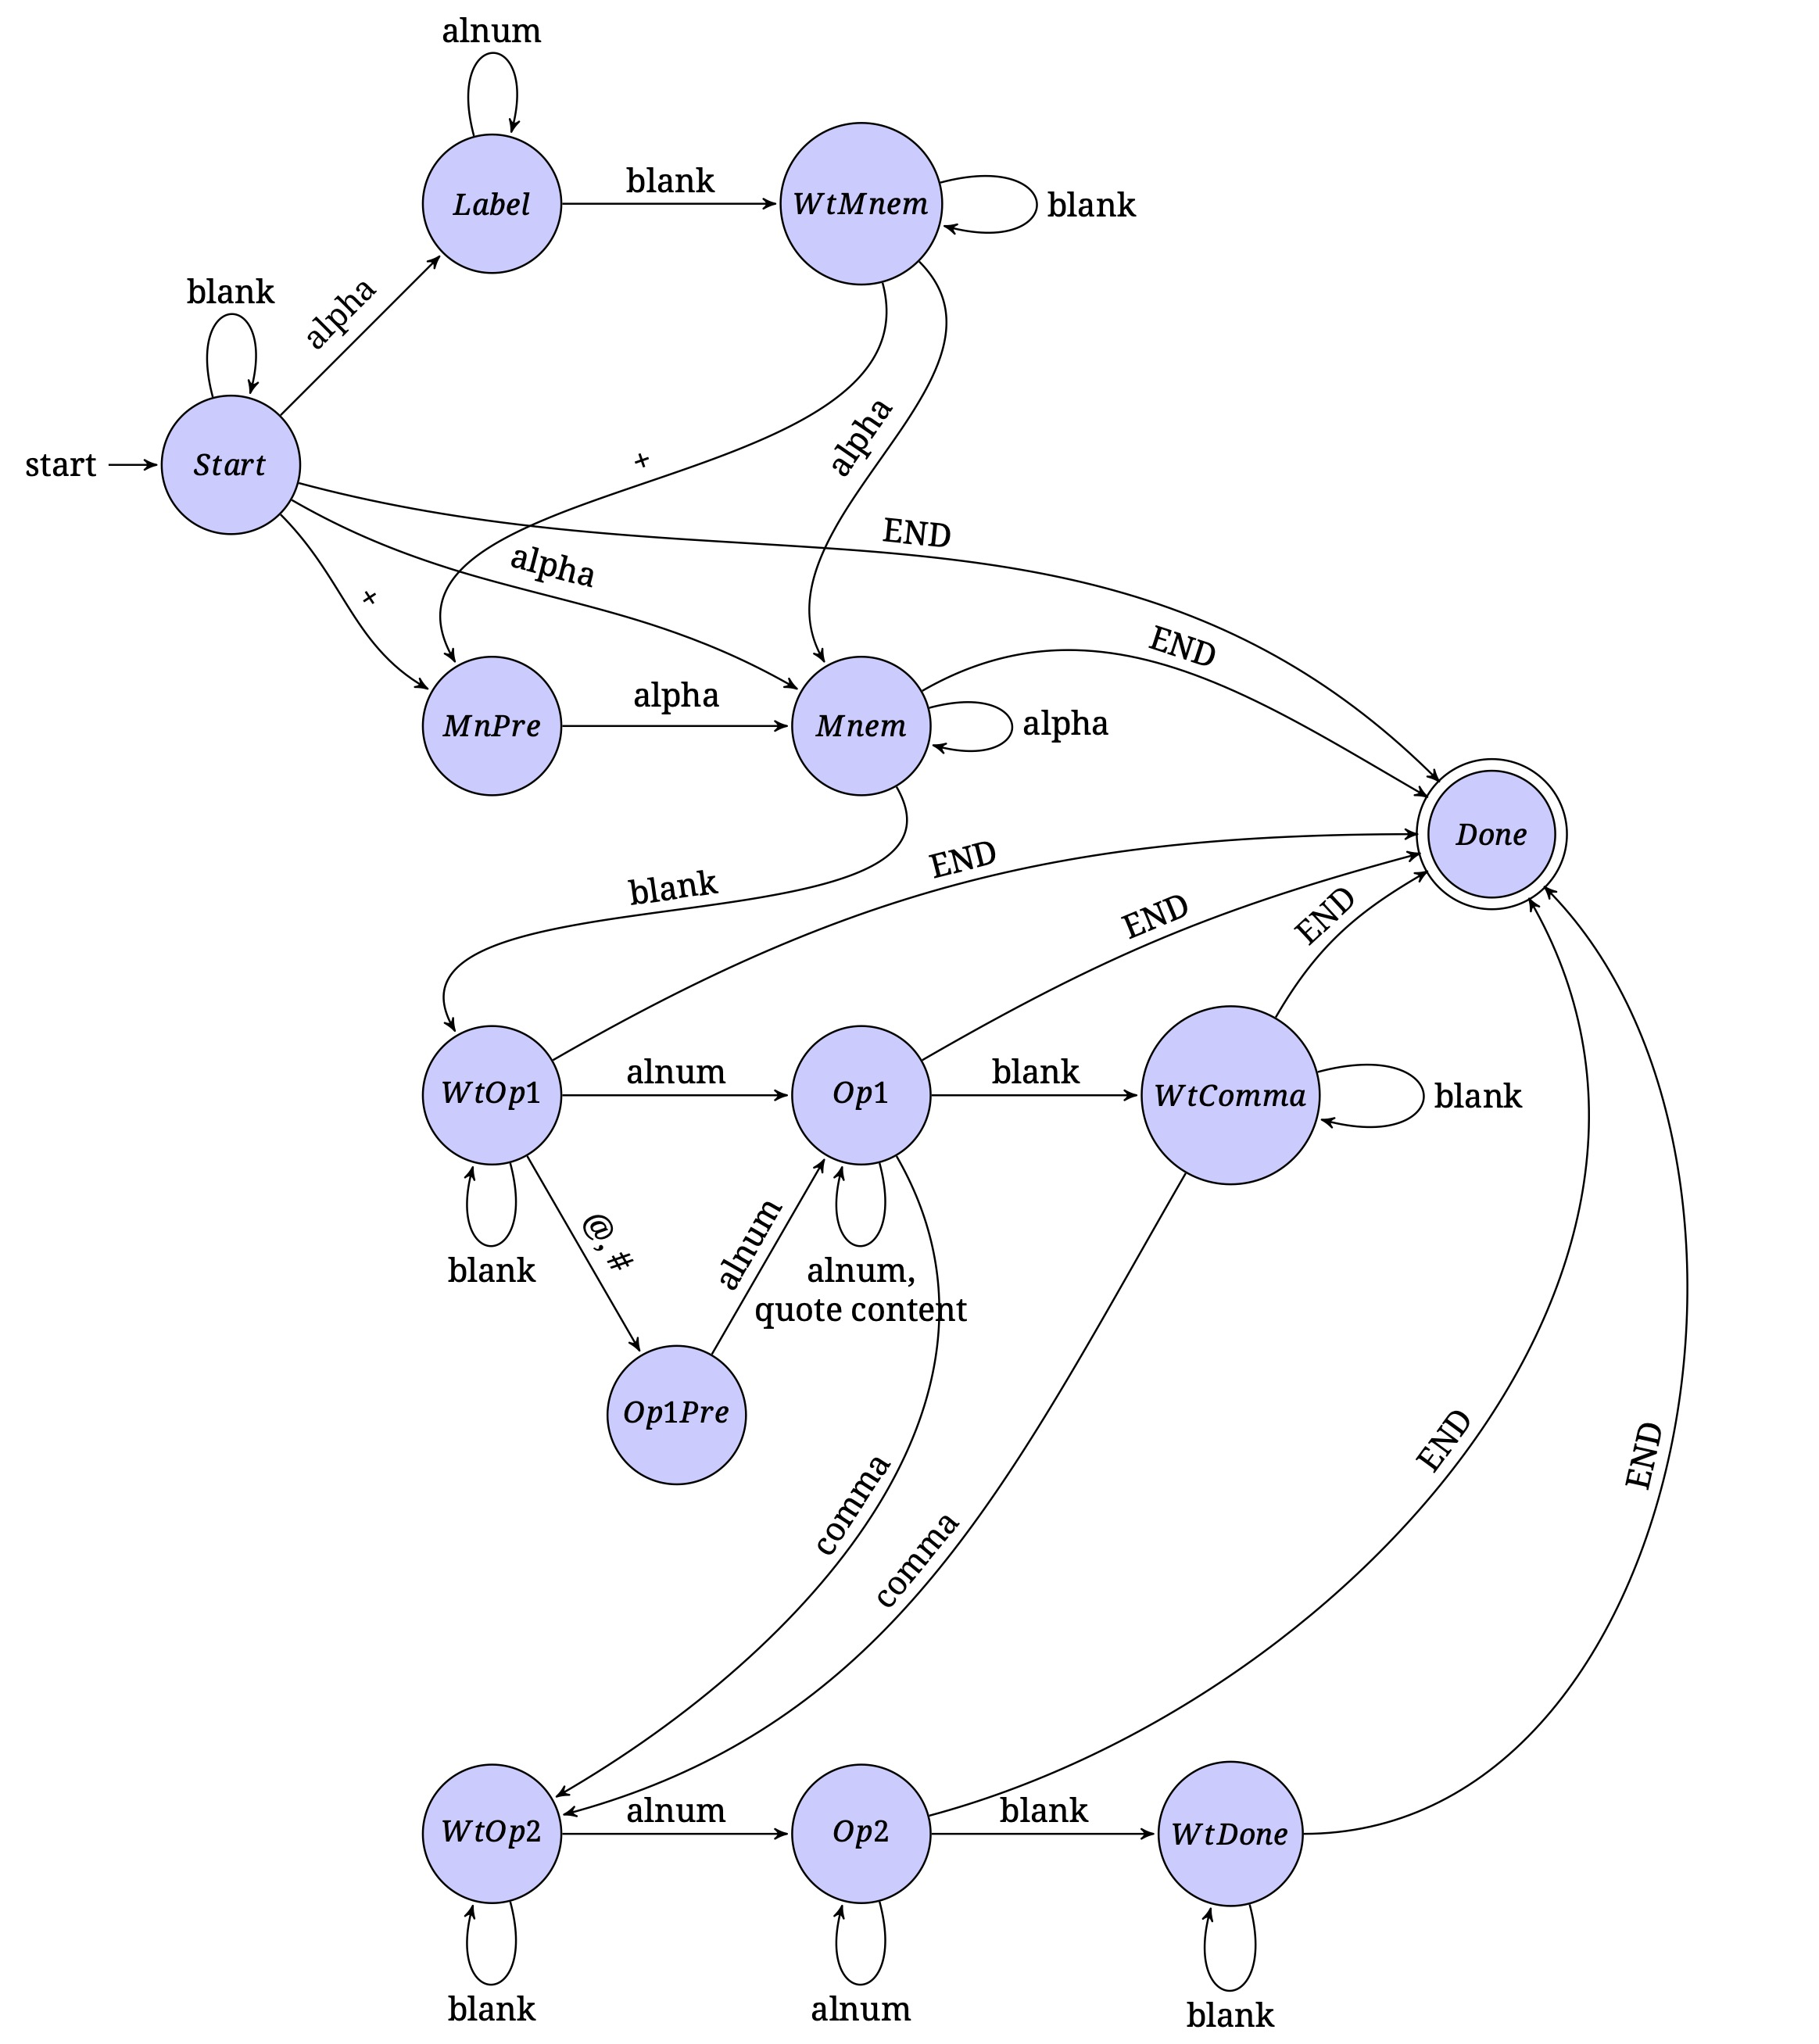
\includegraphics[width=0.8\textwidth]{docs/fsm.jpg}
        \caption{有限狀態機（FSM）狀態轉移圖示。}
        \label{fig:fsm}
    \end{center}

    其中 $Wt$ 代表等待（Wait），$Pre$ 代表前綴（Prefix），$Mnem, Mn$ 代表助記符（Mnemonic），$Op$ 代表運算元（Operand）。
\end{figure}
